\section{User interfaces}

Most definitely, every reader has interacted with a computer before. But most likely there was no
direct interaction with the kernel. Not only is it tedious to interact with the kernel but also
extremely time consuming. This is where user interfaces (UIs) come to help.

\subsection{The shell}

The shell is the outermost layer of an OS. Users interact with the shell to start, pause and quit
programs. Most readers will be familiar with a \textit{graphical user interface}, GUI for short. GUIs come
with a desktop and a taskbar where programs can be started by clicking on the icon. A GUI provides
graphical windows that can be moved around with a mouse or a trackpad. Fortunately for users GUIs
hide away a lot of the complexity of the OS. Users might think that their browser such as Chrome or
Firefox is the only program that is running when they click their browsers icon in the taskbar. But
actually many other programs are already running before users even get to see their desktops taskbar,
let alone their login screen. Traditionally computers were accessed using a \textit{command line interface}
(CLI) that only provide monospaced character output, sometimes even only in monochrome, meaning one
color on black background. CLIs don't use a lot of system resources. This is due to the fundamental
difference in architecture between GUIs and CLIs.

\subsection{Windowing systems and GUIs}

GUIs are made of programs that facilitate windows, icons, menus and pointing with a cursor. One of 
its components is a program called the \textit{display server}. It is responsible for the communication between
all the programs that have a graphical output. This communication occurs through a \textit{display server protocol}
and the programs communicating with the display server are its clients. In windowing systems every
program has its own \textit{window buffer}. It is a dedicated area in memory that the graphical program can
render its own graphical output to. Whenever the program has finished rendering its own window it will
message the display server over the aforementioned display server protocol. The display server has
access to all the window buffers and creates a single frame for a computer screen out of all the
windows in a routine called \textit{compositing}. In some windowing systems there is a separate process that
composits the windows, namely a \textitöwindow manager}. The window manager, as a separate process or not,
draws the windows and their borders and may add effects such as transparency or gaussian blur. It will
factor in the Z-order which is the ordering of windows from back to front and draw the windows in to a 
frame buffer accordingly. As a last step it will also draw the cursor at the cursor position.
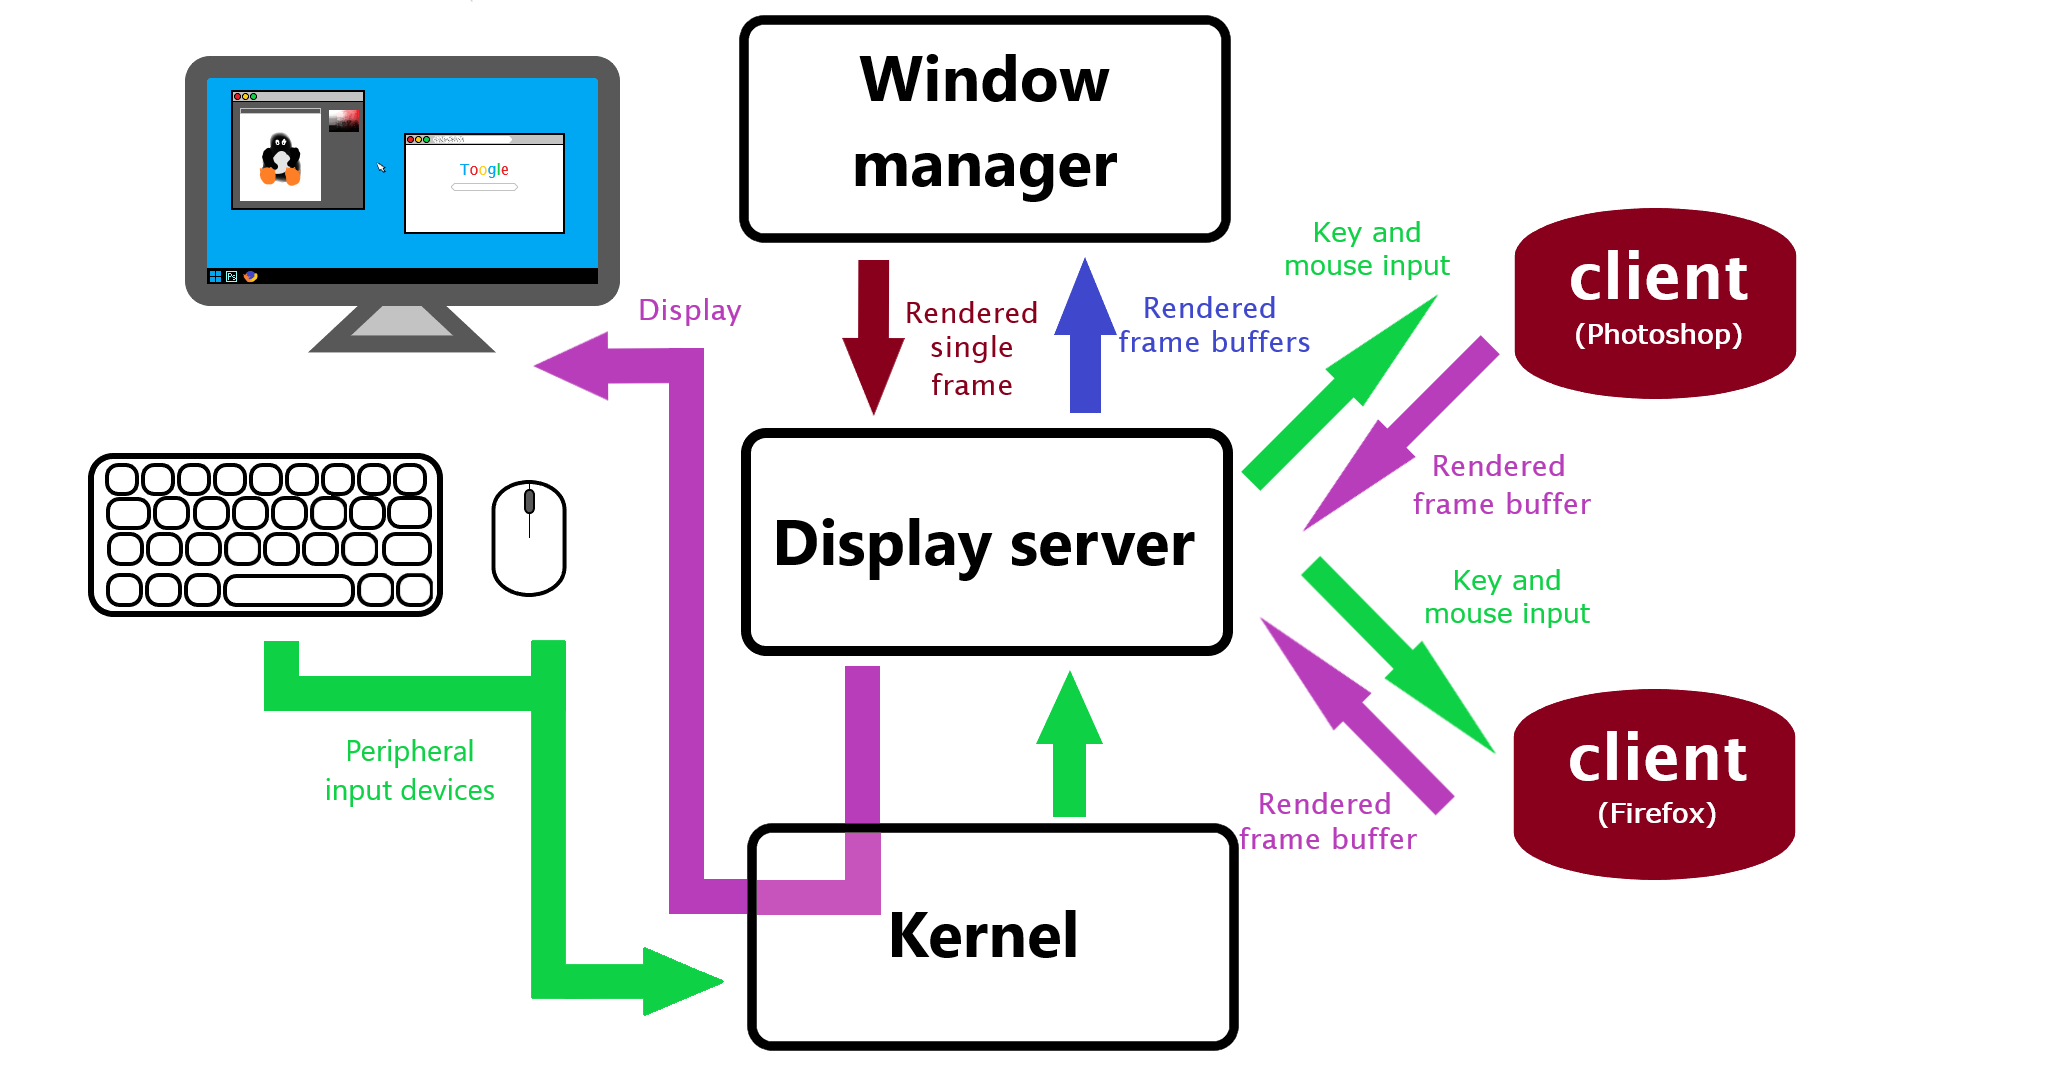
\includegraphics{displayserver.png}

\subsubsection{Rendering}
Every program is responsible for rendering its own window buffer. This includes but is not limited to:
\begin{itemize}
\item font rendering
\item drawing of images
\item widgets such as text input fields and checkboxes
\end{itemize}

Together they form the magnificent windows and desktop background pictures we know and love. But rendering
is a (relatively) time consuming and complex process. However, most windowing systems will also include 
font rendering tools that are optimized for speed and accuracy. There is no point in every program having 
its own font rendering tool as there is no point in reinventing the wheel. There are some other tools for
faster rendering of shapes and images provided by either the display server itself or an extension
thereof.


GUIs are heavily reliant on mouse input to drag, resize and reordering windows but keyboard input
is just as important for a enjoyable user experience. There may be multiple windows running
simultaneously and all of them are waiting for user input. Input from external devices is handled by the
kernel. The display manager more or less exclusively acquires the right to the system input
and decides whom to send key strokes or pointer events such as scrolling or rightclicking. Additionaly,
the display server will check if the input received from the kernel requires a window focus change.
Focus indicates the selected window which will get user input. If the display server notices that
the user has clicked on a window outside of the current window with focus it will transfer the focus
to the new window and change its Z-order to bring it to the front.
The display manager will also check wether a click has been made on one of the programs window bar
buttons such as the close, minimize or maximize buttons or if the window has been resized by clicking
and draging the border. It will then tell the program that it has been resized and the program will
redraw its buffer according to the new dimensions of its window and then communicate the changes to the
display server.

\subsection{CLI}

Command line interfaces are a text-only interface that put emphasis on speed, practicality and
efficency. The are purely controlled by the keyboard and are operated by entering
commands into to the command prompt. The commands are processed by a program called a \textit{command
interpreter}. The command line interpreter is a program that awaits
textual commands to invoke a program. A program can be started by typing its name into the shell. The
shell evaluates the input of the user. Valid input can be one of the following:
\begin{itemize}
	\item A shell built-in command
	\item Full or relative path of an executable program or a program name with its path in the \textbf{PATH} \textit{environment variable}.
\item Interactive scripting keywoards 
\end{itemize}

\subsubsection{Shell built-ins}

Many functionalities that are available to a user are \textit{programs}. Some of those programs do such primitive
tasks and encapsulating them in a separate program (i.e. not part of the command line interpreter) would
be too much of an overhead. These small functionalities are called \textit{commands} instead of program because
they are provided by the command line interpreter itself. Examples of such commands are \textit{cd/chdir}, which
is used to change the \textit{current working directory} or \textit{help}, which is used to display helpful information
about the command line interpreter. \footnote{Shell, from: Wikimili, \today \\ https://wikimili.com/en/Shell_(computing)}

\subsubsection{Environment variables}

Typing out full path names of executables is very annoying when invoking commands, especially if there
are multiple directories where executables are located. Operating system designers came up with a clever
solution to circumvent the inconvenience. Every process is assigned \textit{environment variables}. They are
made of \textbf{name -> value} pairs. Environment variables are passed from a parent process to its child.
Every process can change its own environment variables and pass them on to its child processes if it
chooses so. Environment variables are extremely useful in context of CLIs. On of those environment
variables is '´PATH´'. It is a string with the following format: '`path0:path1:path2:path3:...`' where
path$N$ is an absolute path to a directory and the colon `':'` in unix-like systems or semicolon `';'`
in Windows-family operating systems signifies a separator. When the user enters the name of an 
executable it will check wether it is a full path. If that is not the case the shell will check its
environment variables for `'PATH'` and look at its value. It will check every directory listed in
`'PATH'` sequentally and probe wether an executable with the specified name exists in the directory.
The command line interpreter will let the user know if it fails to find a executable with a matching
name. Environment variables are widely used nowadays but are mostly hidden from users autilizing a GUI.
The GUI will hide away most of the complexity of the OS, one of them being environment variables.


\subsubsection{Scripting}

Users sometimes have more demanding requests of programs they wish to invoke. Users wishing to invoke a
program one hundred times would need to type in the desired programs name a hundred times. Invoking
a program over a hundred times is rather unusual in a GUI environment but in a CLI it may have its
appliances. There are \textbf{shell builtins} to get around this issue. These are tools provided by the shell
(not individual programs) that allow for primitive but nonetheless powerful scripting. Such functionality
can be used by typing in keywords such as `while`, `if`, `else`, `do` and alike. As mentioned,
the command line interpreter is a program and the implementation may vary. Some interpreters have a
slightly different syntax. \footnote{Forsythe: Scripting, \today \\ https://wikimili.com/en/Shell_(computing)}



CLIs appeared in the times of teletype machines that could only display monochrome color output. All
modern monitors are capable of displaying high resolution multi-colored images and todays graphics
accelerated hardware has become cheaper and gotten fast, which resulted in GUIs prevailing over
CLIs. However, CLIs are very convenient for system administrators and automation of routine computer
tasks such as backups. Most graphical OSes come bundled with a \textit{terminal emulator}, a graphical program
running a command line interpreter (such as CMD). This provides flexibility for people who use GUIs for their web
browsing et al. and system administrative tasks or running text-only programs.


\subsection{Remote Access}

As computers incorporated more and more internet capabilities, engineers added functionalities for
\textit{remote access}. This meant that a user connected to a \textit{local area network} (LAN) with his computer
was able to interact with another computer located on the LAN and interact with the remote machine
as it was a local device. 

\subsubsection{Secure shell}

The first type of remote access was a login program listening on the network. It was over a protocol called
telnet and a user was able to connect to another computer running a \textit{telnet server} using a \textit{telnet client}.
However, it was quickly overtaken by a new protocol due to its unencrypted nature: \textbf{SSH}, the \textit{Secure SHell}.
SSH works similar to telnet in a sense of accessing a remote computer. A user can log in to a different
computer running a textit{SSH server} by using a \textit{SSH client}. Unlike telnet, SSH encrypts all internet traffic,
which is crucial when sending passwords over a network. SSH has become a standard today and is widely used to
manage server computers on both local and wide-area networks. \footnote{Secure shell from: CMU, \today \\ https://computing.cs.cmu.edu/security/security-ssh}

\subsubsection{Remote Desktop}

Many programs (such as web browsers) exist only in \textit{graphical mode} and do not support a text-only interface.
However, remote access can also be served in a graphical format. The protocol differs greatly from SSH because
it must additionaly support mouse input and screen output. On the host machine, the display server redirects
the framebuffer output to the client. The client consistently sends keystrokes and mouse events to the display
server. Example of such protocols is the \textit{Remote Desktop Protocol (RDP}.
